\section{Background}

In response to multiple growth factors and cytokines, the
mitogen-activated protein kinases (MAPKs) ERK1 and ERK2 play important
roles in signal transduction pathways that regulate various cellular
processes, which include cell growth, differentiation, gene expression
regulation, and cell development
\cite{kolch2005coordinating,blenis1993signal}. Activation of ERK1 and
ERK2 occurs during the G$_0$/G$_1$ transition and may be required for
progression through the cell cycle
\cite{lavoie1996cyclin,roovers2000integrating}. ERK1 and ERK2 are
present in all cell types, and are evolutionarily conserved,
indicating their importance in cellular signaling pathways
\cite{sugden1997regulation,marshall1994map,robbins1994map}. Given that
MAPK ERK1 interacts with five HIV proteins \cite{fu09}, and MAPK ERK2
has interactions with ten HIV proteins \cite{kolch2005coordinating},
and both kinases participate in multiple cellular processes, it is
likely that it and ERK1 and ERK2 are involved in many steps of HIV
infection \cite{ptak08}.

\subsection{MAPK and HIV infection}

ERK1 and ERK2 have been shown to increase HIV infectivity by
phosphorylating a subset of HIV proteins \cite{yang99}. Inhibiting the
phosphorylation of HIV Vif has impaired, but not stopped HIV
replication \cite{yang99, barraud08}. Prior to HIV replication, the
HIV structural protein matrix (MA) must be phosphorylated by ERK2 to
allow the HIV preintegration complex to translocate to the nucleus,
where viral replication can proceed \cite{bukrinskaya96}. Nef and Tat
have been shown to induce the ERK MAPK cascade
\cite{toschi06,schrager02}. ERK1 and ERK2 phosphorylate HIV Nef, Rev,
and Tat in vitro \cite{yang99}, but the roles of these phosphorylation
events in HIV infectivity remain unknown \cite{yang98}. The inhibition
of MAPK phosphorylation has been shown to decrease HIV infectivity,
indicating that MA and Vif MAPK-directed phosphorylation events might
make good drug targets \cite{yang99,bukrinskaya96}.

\subsection{MAPK substrate docking} 

%% Have MAPK drugs been tried with HIV? Can you target ligand sites with
%% drugs? Are ERK1/2 in siRNA screens? NO. Is the MAPK pathway enriched in
%% virus targeted pathways? NO

Like all MAPKs, ERK1 and ERK2 phosphorylate their substrates at serine
and threonine residues \cite{sugden1997regulation}. Before ERK1 and
ERK1 can phosphorylate their substrates, they must bind to them at
specific docking sites \cite{bardwell09}. Two consensus MAPK substrate
docking patterns have been proposed for eukaryotes, although some
exceptions to these patterns do exist
\cite{puntervoll03,bardwell09}. The Eukaryotic Linear Motif (ELM)
Resource \cite{puntervoll03}, a database of peptide motifs that guide
protein interactions, has developed patterns that represent the two
versions of the MAPK docking site. It refers to these docking sites as
LIG\_MAPK\_1 and LIG\_MAPK\_2.

The LIG\_MAPK\_1, or D-site, pattern has two functional regions: a
string with two or three basic residues and a chain of alternating
hydrophobic residues \cite{bardwell09}. One to six residues maintain
distance between these regions, helping them interact with distinct
regions on MAPKs \cite{bardwell06}. The basic component of the motif
interacts with MAPKs at a patch of acidic residues, called the common
docking (CD) site, while the hydrophobic region of the D-site
interacts with a hydrophobic groove close to the CD site
\cite{liu06}. The LIG\_MAPK\_2 docking site pattern is simply FXFP,
where the letters correspond to amino acids, with X representing any
amino acid. The LIG\_MAPK\_2 docking site is not utilized as a docking
site as much as the D-site \cite{puntervoll03}. Recent work with
small-molecule drugs suggests that the D-site could be targeted to
disrupt its interaction with MAPKs ERK1 and ERK2. Although using
small-molecule drugs to target protein interactions has been difficult
in the past \cite{arkin2004small}, there have been recent advances,
both experimentally \cite{remenyi06} and computationally
\cite{parthasarathi2008approved}, that could be used to target the
docking of MAPK with HIV substrates.

\subsection{Disrupting protein-protein interactions using small-molecule inhibitors}

Most MAPK drugs prevent MAPKs from interacting with ATP by blocking
the conserved ATP binding site. The use of the ATP binding site in
drug development raises concerns about these drugs' lack of
specificity due to similarities among ATP binding sites
\cite{pan09}. New research has suggested that a more specific means of
inhibition may be achieved by preventing MAPK substrate docking using
small-molecule inhibitors \cite{burkhard09,hancock06}. These
protein-protein interaction inhibitors are good drug candidates
because they are often cell permeable, and they are more stable than
peptide inhibitors \cite{thompson1996synthesis}. Experimental studies
have found small-molecule inhibitors for some protein
interactions. For instance, one study found small-molecule inhibitors
that stopped apoptosis by blocking the interaction of the Bak BH3
motif with members of the Bcl-2 family
\cite{degterev2001identification}. Another study used computational
structure modeling and docking to identify small-molecule inhibitors
that blocked calcineruin-NFAT signaling by disrupting docking between
the calcineruin phosphatase and its substrate
\cite{remenyi06,roehrl2004selective}.

Experimental approaches for identifying small-molecule inhibitors of
protein binding are costly and labor intensive
\cite{degterev2001identification,arkin2004small}. Computationally
aided studies like the calcineruin inhibitor development help to
reduce experimental drug development by identifying protein
interaction sites, and finding small-molecules that will act on these
sites \cite{remenyi06}. A pure computational study sought to aid
future work concerned with using small-molecule drugs to disrupt
protein-protein interactions \cite{parthasarathi2008approved}. By
computationally testing all U.S.\ Food and Drug Administration
approved small-molecule drugs for their ability to disrupt protein
complexes with known peptide binding sites and available 3D
structures, the authors behind the study identified a number of drugs
that prevented peptide motif mediated interactions for nuclear
receptors and peroxisome components. With knowledge of docking sites
on HIV, small-molecule inhibitors might also be developed to disrupt
HIV protein phosphorylation by MAPKs, which may hinder HIV
replication. However, care must be taken when designing HIV drugs
because of strain diversity.

%% An ERK inhibitor, FR180204, was deemed to selectively inhibit ERK1/2
%% when it failed to inhibit seven other kinases \cite{ohori05}. However,
%% with nearly 500 kinases left to test \cite{manning02}, specificity is
%% still a concern.

As addressed in Chapter \ref{chapter:prelude}, HIV has been classified
into different strains, or subtypes, and often these strains combine
into recombinant forms \cite{taylor08}. Five subtypes and two
recombinants are present in at least 2.5\% of the world population,
making subtype diversity an issue for drug and vaccine design. HIV
subtype has been found to influence transmission and disease
progression \cite{taylor08}. The presence and absence of short peptide
motifs on HIV proteins has been correlated with patient response to
certain therapies \cite{dampier09}, indicating that differential
docking site usage among strains should be considered when designing
drugs.

In this study, we examine MAPKs ERK1/2 docking with HIV proteins from a
drug design perspective using multiple alignments of HIV protein
sequences taken from different patients, and classified according to
subtype. We find that only HIV Nef has docking site pattern hits that
cover the majority of protein sequences of the most common HIV
subtypes (A1, B, and C). However, the structure of Nef and our in
silico simulations show that docking at these site is unlikely. Some
of the most frequently observed subtypes of HIV proteins MA, Tat, and
Vif are missing the docking pattern most often observed in eukaryotic
MAPK substrates, whereas HIV Rev does not show the docking pattern on
any subtypes. To explain MAPK docking with HIV proteins in a subtype,
or strain, independent manner, we impose slight revisions on the MAPK
docking patterns described in the ELM Resource. One such revised motif
is present in all major subtypes of HIV proteins known to be
phosphorylated by ERK1/2, and is statistically enriched among the
substrates of ERK1/2. The use of in silico docking indicates the
plausibility of the candidate motifs as HIV protein docking sites for
ERK1. Our results provide a first step towards identifying the docking
site motifs on HIV proteins and await experimental verification.

%% This study has even more importance as a study of host peptide motifs
%% on virus proteins.

\section{Results}

\subsection{Consensus MAPK docking sites on human proteins}

\begin{table}\footnotesize
\begin{center}
  \begin{tabular}{|l|c|c|c|c|}
  \hline
  Motif	& Pattern & Phos(\%) & ERK(\%) & p-val\\
  \hline
Da &	[KR]\{0,2\}[KR].\{0,2\}[KR].\{2,4\}[ILVM].[ILVF] & 558 (43) & 56 (45) & 0.299\\
Db&	[KR]\{2,3\}.\{1,6\}[ILVM].[ILVF]&	513 (39)&	51 (41)&	0.348\\
Da U Db&	-&	620 (48)&	69 (56)&	0.030\\
Dc&	[KR].\{2,6\}[ILVM].[ILVF]&	841 (65)&	92 (75)&	0.007\\
Dd&	[KR].\{1,3\}[KR]\{2\}&	694 (53)&	70 (57)&	0.231\\
\hline
  \end{tabular}
\end{center}
\caption[MAPK docking pattern hits on human proteins]{\small Using
  each of the MAPK docking site patterns, we scanned phosphorylated
  substrates in the Database of Post Translational Modifications
  (dbPTM) \cite{lee06}. We show the number of phosphorylated
  substrates with pattern matches (Phos column) as well as results for
  ERK1/2 substrates (ERK column). We used Fisher's exact test to
  calculate a p-value for the enrichment of pattern hits on ERK1/2
  substrates compared to all other phosphorylated proteins. The
  standard docking site patterns, Da and Db, were not enriched on
  ERK1/2 substrates, but the union of these patterns, Da U Db, was
  enriched. Dc, but not Dd, was found to be enriched on ERK1/2
  substrates. \label{tbl:plosONE1:patterns}}
\end{table}



As described above, MAPK docking site sequences, found in most
eukaryotic MAPK substrates, are presented as two distinct patterns,
dubbed LIG\_MAPK\_1 and LIG\_MAPK\_2, by the Eukaryotic Linear Motif
(ELM) Resource. The LIG\_MAPK\_2 pattern was not considered in this
analysis because it was not found to be enriched in human ERK1/2
substrates, and it was not expressed by the HIV proteome (data not
shown). The LIG\_MAPK\_1, or D-site, pattern has two functional
regions: a string with two or three basic residues and a chain of
alternating hydrophobic residues \cite{bardwell09}. One to six
residues maintain distance between these regions, helping them
interact with distinct regions on MAPKs \cite{bardwell06}. The ELM
Resource describes one version of the D-site (Da), while the current
literature contains another frequently observed MAPK docking motif
(Db), with a pattern similar, but not identical, to that of Da
\cite{bardwell09}. Both of the Da and Db motifs have the same
biochemical foundations (Table \ref{tbl:plosONE1:patterns}). The
patterns, or regular expressions, of docking motifs Da and Db were
constructed to account for MAPK docking sites observed in multiple
eukaryotic species \cite{puntervoll03}. Nonetheless, these motifs can
serve as starting templates for the discovery of HIV sequences
involved in docking to MAPKs ERK1/2.

To determine the usage of MAPK docking sites in the human proteome, we
scanned proteins with documented phosphorylation sites \cite{lee06}
and ERK1/2 substrates \cite{lee06} with the Da and Db docking site
patterns. Since functional peptide motifs tend occur in unstructured
regions of proteins \cite{gould2010elm}, tools for motif annotation
and discovery do not scan protein regions containing domains
\cite{puntervoll03,neduva06nuc,edwards07}. To accomplish this domain
filtering, we removed pattern hits falling in Pfam domains
\cite{finn08} in a manner similar to the one used by the ELM Resource
\cite{puntervoll03}. The results presented in Table
\ref{tbl:plosONE1:patterns} indicated that a combined pattern
representing both Da and Db docking motifs, referred to as the Da U Db
pattern, was enriched on ERK1/2 substrates relative to all
phosphorylated substrates (p-value $<$ 0.03). This statistical
enrichment provided evidence supporting the validity of the Da U Db
pattern as the MAPK docking site motif among human proteins.

\subsection{MAPK docking sites on HIV proteins}

\begin{table}\footnotesize
\begin{center}
\begin{tabular}{|l|c|c|c|c||l|c|c|c|c|}
\hline
\multicolumn{5}{|c||}{A (Da)} & \multicolumn{5}{|c|}{B (Db)}\\
\hline
VP & A1 & B & C & Total & VP & A1 & B & C & Total\\
\hline
MA&	6&	14&	50&	34&	MA&	1&	1&	1&	1\\
Nef&	97&	89&	98&	93&	Nef&	96&	89&	91&	90\\
Rev&	1&	9&	1&	3&	Rev&	0&	0&	1&	0\\
Tat&	0&	0&	0&	0&	Tat&	67&	91&	44&	59\\
Vif&	92&	6&	97&	50&	Vif&	1&	5&	61&	27\\
\hline
\hline
\multicolumn{5}{|c||}{C (Dc)} & \multicolumn{5}{|c|}{D (Dd)}\\
\hline
VP & A1 & B & C & Total & VP & A1 & B & C & Total\\
MA&	95&	96&	96&	96&	MA&	95&	99&	97&	97\\
Nef&	100&	100&	100&	100&	Nef&	60&	92&	86&	87\\
Rev&	100&	99&	96&	97&	Rev&	100&	100&	100&	100\\
Tat&	69&	93&	45&	61&	Tat&	100&	99&	100&	99\\
Vif&	100&	100&	100&	100&	Vif&	92&	87&	100&	92\\
\hline
  \end{tabular}
\end{center}
\caption[MAPK docking pattern hits on HIV proteins]{\small We searched sequences of HIV proteins using the four MAPK docking site patterns in Table \ref{tbl:plosONE1:patterns}. Here we present the percentages of HIV subtype sequences with these docking site patterns. The Da and Db  patterns were found on the majority of Nef sequences, but they were missing from some subtypes of the other HIV proteins. The Dc pattern occurred on the majority of MA, Nef, Rev, and Vif subtypes. The Dd  motif had hits on most sequences of all HIV proteins. \label{tbl:plosONE2:percents}}
\end{table}



Since MAPKs ERK1 and ERK2 substrates were statistically enriched with MAPK
docking motifs, we hypothesized that the presence of these docking
sites on most sequences of HIV proteins MA, Nef, Rev, Tat, and Vif
would explain their reported phosphorylation by ERK1 and
ERK2. Therefore, we searched for the MAPK docking site patterns on HIV
sequences gathered from the Los Alamos National Lab (LANL) HIV
Sequence Database (http://www.hiv.lanl.gov/), which contains thousands
of sequences spanning multiple subtypes and recombinant forms. In this
analysis, we considered HIV strains with at least 50 sequences for all
HIV proteins known to interact with ERK1/2, leaving three strains to
consider: A1, B, and C. Having at least 50 sequences for each strain
provided us with enough sequence diversity to assess the conservation
of docking pattern hits. Subtypes A1, B, and C are responsible for the
majority of the HIV infection around the globe \cite{hemelarr06},
making them appropriate for this study. Figure \ref{fig:plos1:fig1}
shows the Da and Db motif annotations on multiple sequence alignments
of HIV proteins, and Table \ref{tbl:plosONE2:percents} shows the
percentages of HIV subtype sequences with docking site matches. The
results showed a subtype dependence for the annotations of the Da and
Db patterns along HIV proteins.

\begin{figure}
\begin{center}
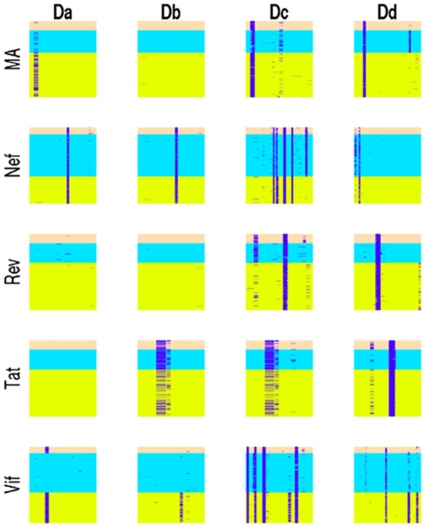
\includegraphics[scale=0.9]{figs/plos1_1}
\end{center}
\caption[MAPK docking site pattern hits on HIV proteins]{\small Hits
  for the standard MAPK docking sites, Da and Db, and the proposed
  MAPK docking sites patterns, Dc and Dd, are annotated in purple on
  multiple sequence alignments of HIV proteins MA, Nef, Rev, Tat, and
  Vif. Subtypes in each alignment are represented by different colors:
  A1 is pink, B is blue, and C is green. Note that motif annotations
  occur in roughly the same position within a virus
  subtype. \label{fig:plos1:fig1}}
\end{figure}

More than 90\% of Nef sequences had the Da motif regardless of
subtype, but this motif was absent on most Tat and Rev sequences. Vif
subtypes A1 and C, but not B, expressed the Da motif. On the other
hand, the Db motif was present on Nef, Tat, and subtype C of Vif, but
was absent on MA and Rev. The Da and Db motifs occupied different
spatial positions along the HIV proteins. The data shown in Figure
\ref{fig:plos1:fig1} suggested Nef was the only HIV protein for which
phosphorylation by ERK1 and ERK2 could be explained by a standard
docking site. However, after examining a map of solvent inaccessible
residues on Nef \cite{arold2001dynamic}, we found that the Db motif
hit had its last residue in a buried region of the protein. Further
investigation using in silico docking revealed that both the Nef Da
and Db motif hits could not serve as MAPK docking sites (see
Methods). Docking at these sites placed the MAPK active site too far
from the three possible phosphorylation sites on Nef (Figure
\ref{fig:plos1:new}).

\begin{figure}
\begin{center}
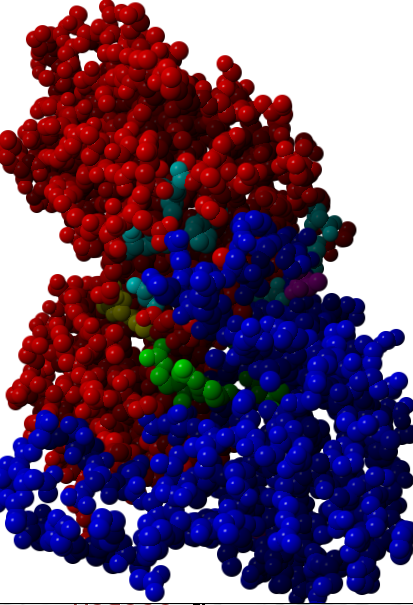
\includegraphics[scale=0.9]{figs/plos1_new_6}
\end{center}
\caption[Docking between MAPK ERK1 and HIV Nef]{\small In silico
  docking of MAPK ERK1 (red) and HIV Nef (blue) at the MAPK docking
  groove (cyan) and the standard docking motif hit on Nef (green) did
  not align the active site of ERK1 (yellow) with any of the three
  possible Nef phosphorylation site (magenta). This suggested that the
  standard docking site pattern match on Nef did not function as the
  real docking site for ERK1. \label{fig:plos1:new}}
\end{figure}

Next we revised the Da and Db regular expressions in an attempt to
find a motif that would be present on all major subtypes of HIV
proteins known to interact with human MAPKs ERK1 and ERK2. We looked
at sequences of HIV proteins without a docking motif coincident with
the spatial position of the standard motifs. Specifically, we looked
at regions along MA and Vif that aligned with the Da motif, as well as
regions of Tat and Vif that aligned with the Db motif, but were not
annotated with the motif (Figure \ref{fig:plos1:fig1}). The absence of
the Da motif in subtypes A1 and C of MA and subtype B of Vif was
caused by a missing basic residue. The absence of Db in some subtypes
appeared to be due to mutated hydrophobic residues. Taking cues from
these perturbations, we designed a new regular expression for a
candidate MAPK docking motif along HIV proteins (Table
\ref{tbl:plosONE1:patterns}), and represented this motif with the
symbol Dc. The motif Dc turned out to be present on HIV proteins Nef,
Rev, Tat, Vif, and MA in a relatively subtype independent manner
(Figure \ref{fig:plos1:fig1}). We assessed the significance of Dc
motif conservation on HIV proteins by comparing it with the
conservation found on random protein sequences (see Methods). We found
that Dc was significantly conserved on all HIV MAPK substrates
compared to random HIV protein sequences (p-value $<$ 0.05).

We also considered whether or not an infrequently observed MAPK
docking motif among human proteins could serve as an HIV
subtype-independent MAPK docking site. The docking site pattern for
MAPK with thyroid hormone receptor-beta1 (TR$\beta$1) is KGFFRR, where
letters represent amino acids. The motif is known to be fully
functional, and yet it is missing the hydrophobic portion of the Da
and Db motifs \cite{lin03}. Furthermore, mutational studies showed
that only the first and final two basic residues were required for
docking, yielding the pattern KXXXRR, where X represents any amino
acid \cite{lin03}. Scanning this motif along the HIV proteome provided
new hits, but did not have sufficient coverage along MA, Rev, Tat, and
Vif subtypes. We expanded this pattern to include all basic residues
in the first and final two amino acids, and allowed variation in the
distance between the basic components, resulting in motif Dd, with the
regular expression given in Table \ref{tbl:plosONE1:patterns}. We used
this new pattern to scan multiple alignments of HIV proteins, and
found hits on the majority of sequences for all HIV proteins known to
interact with MAPK (Figure \ref{fig:plos1:fig1} and Table
\ref{tbl:plosONE2:percents}). As with the Dc motif, we found the
conservation of the Dd motif on HIV MAPK substrates to be significant
(p-value $<$ 0.05) when compared to Dd motif conservation on random
protein sequences(see Methods).

%% This significant conservation of docking motifs was not observed for
%% the standard docking motifs Da and Db for all HIV MAPK substrates.

\begin{figure}
\begin{center}
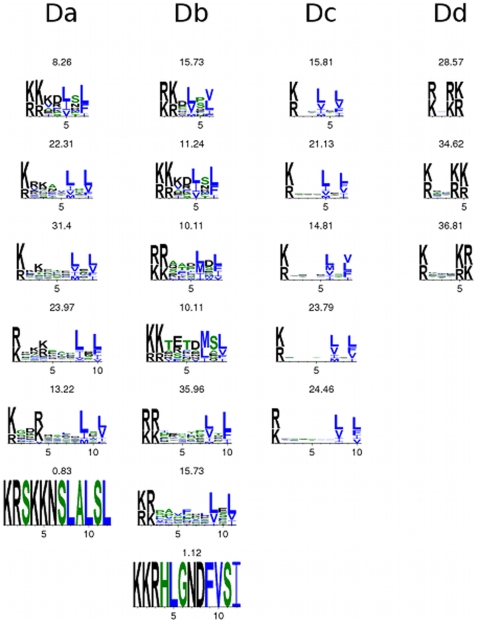
\includegraphics[scale=0.75]{figs/plos1_2}
\end{center}
\caption[Human sequence logos]{\small For the four MAPK docking sites
  in the study, we show sequence logos for hits on human proteins. The
  motifs used here allowed matches with varying lengths. The
  percentage of motif instances of a certain length is shown above
  each logo. \label{fig:plos1:fig2}}
\end{figure}

\begin{figure}
\begin{center}
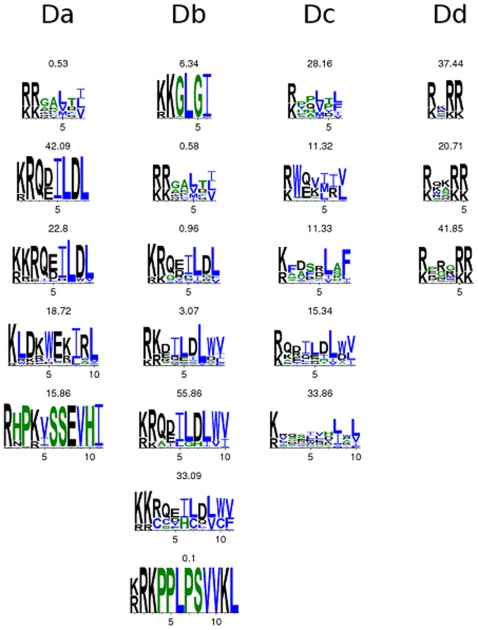
\includegraphics[scale=0.7]{figs/plos1_3}
\end{center}
\caption[HIV Sequence logos]{\small Here we show sequence logos for
  MAPK docking site motif hits on HIV proteins MA, Nef, Rev, Tat, and
  Vif. For each MAPK docking site motif, we gathered all hits on all
  HIV proteins and constructed sequence logos for hits with the same
  length. The percentage of motif instances of a certain length is
  shown above each logo. \label{fig:plos1:fig3}}
\end{figure}

The specific sequences matched by MAPK docking motif patterns can be
different in human and HIV proteins, and this was best observed by
constructing sequence logos from the motif hits on human (Figure
\ref{fig:plos1:fig2}) and HIV (Figure \ref{fig:plos1:fig3}) proteins
known to be phosphorylated by MAPKs ERK1 and ERK2. It was clear from
Figures \ref{fig:plos1:fig2} and ​\ref{fig:plos1:fig3} that the residue
usage for motifs Da, Db, and Dc was similar because all motif hits had
basic residues followed by hydrophobic residues. This similar
biochemical foundation explained why the candidate docking motif Dc
was coincident with Da or Db in the HIV proteome. Our computations
based on Fisher's exact test showed the Dc motif to be statistically
enriched on ERK1/2 binding partners (Table
\ref{tbl:plosONE1:patterns}). The fact that the Da, Db, Dc motif hits
on HIV proteins allow less variation in the spacing residues makes it
possible to target these regions with small-molecule drugs while
preserving host ERK1/2 activity. The Dd motif had more or less the
same residue usage in human and HIV proteins. This motif is a simple
one, and was not statistically enriched among ERK1/2 substrates (Table
\ref{tbl:plosONE1:patterns}).

\subsection{Candidate docking motifs on HIV Nef}

Focusing on ERK1/2 phosphorylation of HIV Nef, we found that neither
of the standard Da and Db docking motifs were supported by in silico
docking (see Methods), and the Db motif failed the solvent
accessibility test. This suggested that one of our alternative docking
motifs could serve as a potential docking site. Using the solvent
accessibility test, we found that none of the Dc pattern hits were
likely MAPK docking site candidates, as each one had at least one
buried residue. Only the initial N-terminal Dd pattern hit did not
overlap with a buried residue. Unfortunately, we were unable to find a
Nef protein structure that had both this Dd pattern hit and the
proposed Nef phosphorylation sites, so in silico docking could not be
performed. Testing the functionality of this proposed site awaits
further experimentation.

\subsection{Candidate docking motifs on the HIV protein matrix are supported by structures}

\begin{figure}
\begin{center}
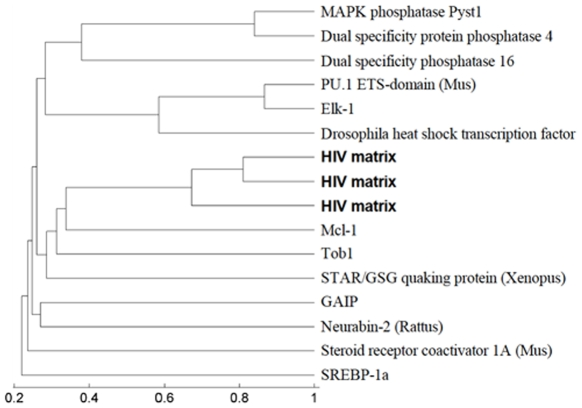
\includegraphics[scale=0.8]{figs/plos1_4}
\end{center}
\caption[MAPK substrate hierarchy]{\small Here we present UPGMA
  clustering of HIV MA proteins and ERK1/2 substrates by pairwise
  structural alignment TM-scores. All substrates are human proteins
  unless otherwise indicated. The HIV MA proteins are shown in
  bold. \label{fig:plos1:fig4}}
\end{figure}

In order to further support the feasibility of our new docking
patterns as MAPK docking sites, we compared the structures of the HIV
matrix protein to those of ERK1/2 substrates. We chose MA in this
comparison due to the availability of multiple structures for this
protein. Figure \ref{fig:plos1:fig4} shows the hierarchical clustering
of the HIV MA proteins and ERK1/2 substrates (with known structures)
by their pairwise structural similarity, as measured by the
TM-score. As explained in the methods section, the TM-score is a
normalized measure of structural similarity that ranges between 0 and
1, where a score above 0.20 is considered significant
\cite{zhang04}. As expected by their 90\% sequence similarity, the HIV
MA proteins (shown in bold in Figure \ref{fig:plos1:fig4}) were
clustered together at a high TM-score (0.65). Surprisingly, some of
the human ERK1/2 substrates (specifically, Mcl-1, Tob1, and the
Xenopus STAR/GSG quaking protein) were found to be structurally more
similar to HIV MA proteins than they were to other ERK1/2
substrates. These results were consistent with experimental data
showing binding between ERK1/2 and HIV MA.

\begin{figure}
\begin{center}
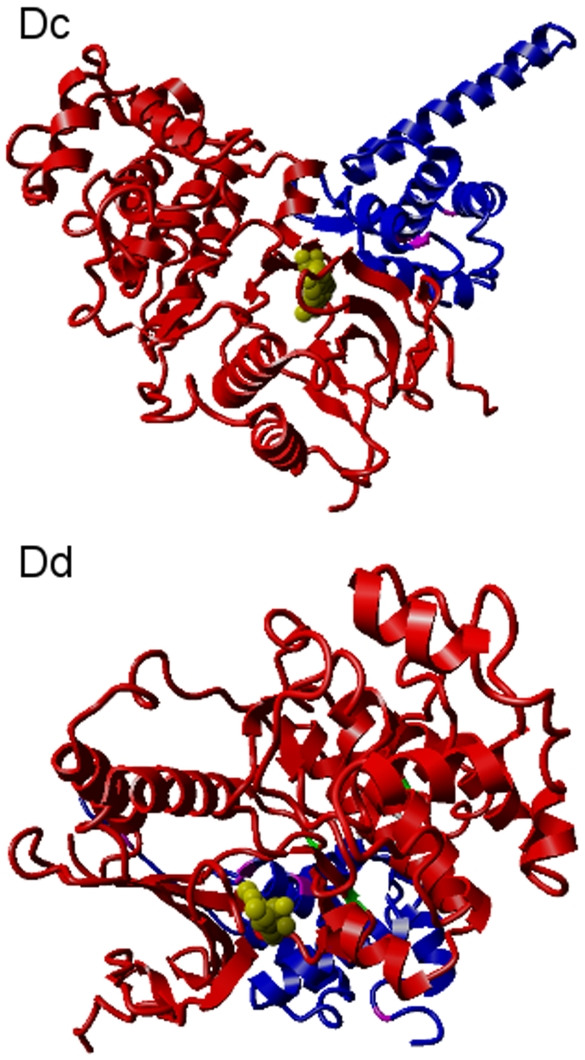
\includegraphics[scale=0.4]{figs/plos1_5}
\end{center}
\caption[Docking between MAPK ERK1 and HIV MA]{\small In silico docking was
  performed using ZDOCK by forcing ERK1 (red) to dock at the Dc and Dd
  motifs on HIV MA (blue). In the upper panel, docking was forced to
  occur between the hydrophobic tail of the Dc motif on MA and the
  hydrophobic docking groove of ERK1. The lower panel shows the
  resulting complex when docking was forced between the basic residues
  of Dd on MA and the CD site of ERK1. The ATP binding site of ERK1
  interacts with MAPK inhibitor 5-iodotubericidin (yellow). When the
  Dd docking site on MA (green) was forced to interact with ERK1,
  serine phosphorylation sites (magenta) on ERK1 were positioned in
  close proximity to the ERK1 ATP binding
  site.  \label{fig:plos1:fig5}}
\end{figure}

We next performed in silico docking between HIV MA and ERK1 using the
ZDOCK server \cite{chen03}. ZDOCK allows users to force binding
between specific residues. The top panel of Figure
\ref{fig:plos1:fig5} shows ERK1 docked with MA when binding was forced
between the hydrophobic portion of Dc and the hydrophobic groove of
ERK1. The bottom panel of Figure \ref{fig:plos1:fig5} shows ERK1
docked with MA after binding was forced between the Dd motif on MA and
the CD site on ERK1 \cite{kinoshita08}. This figure demonstrates the
close proximity of the MA docking site and the ERK1 docking groove
after both forced docking interactions. The ATP binding site of ERK1 is bound by
the MAPK inhibitor 5-iodotubericidin, colored yellow. Both docking
experiments positioned possible phosphorylation sites on MA close to
the ATP binding site of ERK1, adding additional evidence that the Dc
and Dd patterns on MA could be functional. This was demonstrated in
more detail in YASARA (http://www.yasara.org) scenes of the complexes
\\ (\htmladdnormallink{www.ncbi.nlm.nih.gov/pmc/articles/PMC2812490/bin/pone.0008942.s001.zip}{http://www.ncbi.nlm.nih.gov/pmc/articles/PMC2812490/bin/pone.0008942.s001.zip}).

\section{Discussion}

In this study we have shown that known MAPK docking motifs occur in a
subtype dependent manner on HIV proteins known to interact with human
MAPKs ERK1 and ERK2. MAPK substrate docking is known to facilitate
phosphorylation. While the detailed role of MAPK phosphorylation in
HIV infection has not been established in a clinical setting, ERK1/2
phosphorylation of HIV proteins has been associated with viral
infectivity in a number of in vitro studies, highlighting the
importance of MAPK docking sites in the course of HIV infection. For
this reason, we hypothesized that if MAPK phosphorylation of HIV
proteins was an essential feature of the progression of HIV infection,
then MAPK docking sites along HIV proteins would be subtype
independent. This was our motivation for revising known human MAPK
docking sites for the case of HIV proteins.  Our study suggested two
docking motifs, Dc, and Dd, and showed that these appeared on all
subtypes of HIV proteins phosphorylated by ERK1/2. These motifs shared
biochemical characteristics with motifs used by human proteins that
bind to MAPKs. The Dc motif was missing one basic residue form the
standard docking motifs, while the Dd motif was missing the
hydrophobic portion. The Dd motif had experimental support on human
proteins, while the Dc motif did not. In silico docking experiments
provided evidence supporting the hypothesis that these motifs function
as MAPK docking sites along HIV proteins. One of these candidate
motifs, Dc, was statistically enriched among the binding partners of
ERK1/2. However, the lack of statistical enrichment does not exclude
the possibility of the Dd motif being used as a docking site as well.

Current drugs target MAPK activity, but new drugs based on the HIV
MAPK docking sites might work better. Existing MAPK drugs, like
SB203580, SB202190, and RWJ67657 do not target ERK1/2. FR180204 does
target ERK1/2 activity via the ATP binding site, making it susceptible
to off target effects. New drugs targeting HIV replication by blocking
ERK1/2 phosphorylation of MA and Vif could in theory be incorporated
into existing therapy regimens, making it more difficult for an HIV
strain to acquire the mutations for resistance to all drugs
\cite{deeks03}. By targeting MAPK docking sites, rather than ATP
binding sites, drugs can offer more specificity. There is hope that
few ERK1/2 substrates will be targeted by drugs specific to HIV
docking sequences. Amino acid sequences used by virus and host in the
Dc motif were significantly different (Figure \ref{fig:plos1:fig2} and
Figure \ref{fig:plos1:fig3}) to allow for specific targeting of HIV
proteins with drugs. Moreover, the poor structural alignment of HIV MA
and other ERK1/2 substrates suggests that HIV specific targeting is
possible.

\section{Conclusion}

The standard MAPK docking motifs from the literature could not explain
the interactions of MAPKs ERK1 and ERK2 with all subtypes of HIV
proteins. The two new motifs we introduced as candidate motifs for
ERK1/2 docking were present on subtypes A1, B, and C of HIV proteins
known to interact with MAPK. These sites can be tested by mutating key
docking site residues on HIV proteins, and observing the effect on
their phosphorylation by ERK1 and ERK2. The amino acid composition of
the docking motifs on HIV proteins was different enough from the
composition found on human ERK1/2 substrates to allow for HIV sequence
specific drug targeting using small-molecule drugs. This study can be
extended based on a recent computational method for identifying
U.S.\ Food and Drug Administration approved small-molecule drugs that
prevent protein-protein interactions
\cite{parthasarathi2008approved}. Using our proposed complex of MAPK
ERK1 and the HIV matrix protein (MA), approved small-molecule drugs
can be screen in silico to find those that disrupt the docking between
ERK1 and HIV MA. Further annotation of the proposed docking motifs
awaits experimental verification.

This study has importance beyond interactions between MAPK and HIV
proteins. In Chapter \ref{chapter:predict}, we showed that certain
host peptide motifs, like the MAPK docking site discussed here, are
found to be conserved on HIV protein sequences taken from different
patients. Here we have shown that the transfer of a standard host
peptide motif to virus proteins is not as simple as previously
thought. We had to make modifications to the docking site provided by
the Eukaryotic Linear Motif Resource before we could explain how MAPK
could dock with HIV proteins. The requirement for these modifications
motivates general questions about host motifs on HIV proteins. What
other host peptide motif are missing on HIV proteins due to inadequate
patterns? How is the virus utilization of variant host peptide motif
patterns beneficial to the virus? These questions help in promoting
more studies of virus-host interactions.

\section{Methods}

\subsection{Human and HIV sequences and motifs}

HIV sequence alignments were gathered from the Los Alamos National
Laboratory (LANL) HIV Sequence Database, and processed according to
\cite{evans09}, but here only subtypes A1, B, and C were used. We
gathered 1436 proteins known to be phosphorylated from dbPTM
\cite{lee06}, and found 132 of these were phosphorylated by ERK1/2. We
scanned all sequences with the four regular expressions for MAPK
docking sites. For human proteins, we attempted to rule out false
positive hits in a manner similar to the ELM Resource. We removed any
pattern hits that overlapped with a Pfam domain \cite{finn08}. Pfam
domains were found for all proteins using the default settings for the
stand alone Pfam scan program. Enrichment of docking site pattern hits
on ERK1/2 substrates was calculated with a one-tailed Fisher's exact
test, using phosphorylated dbPTM substrates as a background set.

\subsection{Significance of proposed docking site motif conservation on HIV proteins}

To assess the significance of our proposed MAPK docking motifs, Dc and
Dd, being annotated on most of sequences gathered for HIV proteins MA,
Nef, Rev, Tat, and Vif, we devised a control based on randomly
constructed HIV protein sequences. Here we describe the control for
the HIV matrix protein, but similar steps were used for all HIV
proteins phosphorylated by MAPKs ERK1 and ERK2. Using our total set of
987 MA subtype A1, B, and C protein sequences from the LANL database,
we estimated the probability of amino acid occurrence as well as amino
acid transition probabilities, i.e.\ the probability of seeing amino
acid $\beta$ follow amino acid $\alpha$ in MA protein sequences. We
constructed one random MA protein sequence for every real MA protein
sequence by first sampling an initial amino acid based on the single
amino acid probabilities, and then using the amino acid transition
probabilities to sample subsequent amino acids and build the rest of
the random protein sequence until it was as long as the real one.

We made one hundred sets of random MA protein sequences, each
containing 987 random Nef sequences, and matched all proteins in each
set against patterns for the Dc and Dd docking sites. For each random
protein set, we calculated the conservation of the proposed docking
sites across random MA protein sequences in the set, and compared this
conservation to the docking site conservation observed for real MA
protein sequences from the LANL database. To obtain a p-value for the
conservation of Dc and Dd on real MA protein sequences, we recorded
the number of random sets where the conservation of the proposed
docking site was equal to or greater than the conservation observed
for real MA protein sequences. We found that both Dc and Dd docking
site motifs were significantly conserved compared to random protein
sequences (p-value $<$ 0.05), i.e.\ the proposed docking motifs had
conservation on real MA protein sequences than on random protein
sequences in more than 95 of the random sequence sets. Using a similar
control for HIV Nef, Rev, Tat, and Vif proteins, we found Dc and Dd
motifs to be significantly conserved for all HIV MAPK substrates,
which made it more likely that they were guiding interactions with
MAPKs ERK1 and ERK2.

\subsection{Structure analysis}

We performed a BLAST \cite{altschul90} search on the Protein Data Bank
(PDB) \cite{berman02} to identify known ERK1/2 substrate protein
structures (E-value threshold of E-10). We collected the proteins that
had less than 150 residues, to be comparable to HIV MA in size, and
only kept the top hit in each BLAST result set. A pairwise structural
alignment of each of three MA structures [PDB$\colon$1hiw,
  PDB$\colon$1uph, PDB$\colon$2hmx] against each MAPK substrate
structure was performed using Vorometric \cite{sacan08}. The
alignments were filtered by a TM-score \cite{zhang04} of 0.25,
resulting in 10 ERK1/2 substrate structures. The PDB identifiers for
the 10 substrates are as follows: PDB$\colon$1mkpA - MAPK phosphatase
Pyst1, PDB$\colon$3ezzA - Dual specificity protein phosphatase 4,
PDB$\colon$2vswA - Dual specificity phosphatase 16, PDB$\colon$1pueE -
PU.1 ETS-domain, PDB$\colon$1duxC - Elk-1, PDB$\colon$1hksA -
Drosophila heat shock transcription factor, PDB$\colon$2pqkA - Mcl-1,
PDB$\colon$2z15A - Tob1, PDB$\colon$2bl5A - STAR/GSG quaking protein,
PDB$\colon$1cmzA - GAIP, PDB$\colon$2g5mB - Neurabin-2,
PDB$\colon$1oj5A - Steroid receptor coactivator 1A, PDB$\colon$1am9A -
SREBP-1a.

\subsection{Docking}

Docking in Figure \ref{fig:plos1:new} was performed with the ZDOCK
server (\htmladdnormallink{http://zdock.bu.edu}{http://zdock.bu.edu})
to find the most likely complex of ERK1 [PDB$\colon$2zoqA] and HIV Nef
[PDB$\colon$2nef] when binding was forced between the proposed docking
site on Nef (Arg105, Arg106, Leu110, and Leu112) and the CD site of
ERK1 (Glu98, Asp179, Asp335, and Asp338 \cite{kinoshita08}).

For the top panel of Figure \ref{fig:plos1:fig5}, ZDOCK was also used
to calculate the most probable complex of ERK1 [PDB$\colon$2zoqA] and
HIV MA [PDB$\colon$1uphA] when binding was forced between the
hydrophobic tail residues of the Dc motif on MA (Ile19 and Leu21) and
the hydrophobic docking groove of ERK1 (Thr127, Leu132, Leu138, and
Phe146 \cite{kinoshita08}).

For the bottom panel of Figure \ref{fig:plos1:fig5}, the ZDOCK
server was used to calculate the most probable complex of ERK1
[PDB$\colon$2zoqA] and HIV MA [PDB$\colon$1uphA] when binding was
forced between the basic residues of the Dd motif on MA (Arg22, Lys26,
and Lys27) and the CD site of ERK1.

